\chapter{Conclusion}
\label{conclusion}

\section{Research Questions Revisited}

This section revisted the three research questions defined in Chapter 1.


\textbf{Research Question 1: }\textit{What are the challenges in search-based crash reproduction?}

With this research question, we tried to detect and categorize the challenges in search-based crash reproduction. Since previous evaluations of these techniques contained a limited number of subjects (at most 50 cases), we could not provide a thorough answer only based on existing results. Hence, to take the first step towards answering this research question, we have designed a benchmark, called \crashpack, which includes 200 real-world Java crashes. We have also proposed a new tool, called \exrunner, to conduct extensive experiments on these crashes.

We have made both \crashpack and \exrunner publicly available for two purposes: 
(i) ease the comparison of the existing crash reproduction techniques; and 
(ii) help researchers in analysing and identify the impacting factors in search-based crash reproduction techniques.

We have utilized \exrunner to apply the state-of-the-art automated crash reproduction tool (\evocrash) on all crashes in \jcrashpack. The outcome of this experiment shows that \evocrash is not successful in reproducing more than 50\% of the crashes in \jcrashpack. Hence, we have performed an extensive manual analysis to identify the challenges leading to unsuccessful crash reproduction in this search-based approach. We have characterized the identified challenges into 13 categories. Some of the identified challenges (\eg complex input generation, complex code, \etc) are related to general search-based test generation issues, and the others are specific to crash reproduction (\eg exceptions are captured by try/catch, and nested private calls in the given stack trace).


This research question confirms that there is still space for improvements in search-based crash reproduction and test generation techniques. Despite the undeniable achievements by search-based crash reproduction, it cannot reproduce about 50\% of crashes in \crashpack. 
This research question categorizes the challenges this technique encounters in unsuccessful cases. This categorization indicates that two of the most common search-based crash reproduction issues stem from the general search-based crash reproduction difficulties: Input Data Generatio and Complex Code. These challenges are indicating the complexity of the problem in search-based crash reproduction and test generation. Hence, establishing that using pure randomness, without using any other sources of information, is not enough for the search process to generate complex solutions.


\textbf{Research Question 2: }\textit{Based on the identified challenges, how can we leverage the existing knowl\-edge, carved from information sources, to steer the crash reproduction search process?}


With this research question, we sought to address two of the most common challenges in search-based crash reproduction, identified in Research Question 1: Input Data Generation and Complex Code. For this purpose, this thesis has introduced new techniques, which utilize the pieces of knowledge carved from different information sources such as source code and manually-written tests. In this thesis, we have introduced a novel seeding strategy (Chapter \ref{sec:model_seeding}), a set of helper-objectives (Chapter \ref{sec:moho:introduction}), and a secondary objective (Chapter~\ref{section:bbc:introduction}) to leverage this information in order to improve the effectiveness and efficiency of search-based crash reproduction.

This research question confirms the relevance of Input Data Generation and Complex Code (two common challenges that we have found in Research Question 1) and introduces new techniques and search objectives to address them. Chapters 3 and 4 address the first challenge by introducing a novel seeding strategy (behavioral model seeding) and designing two search helper-objectives (\moho), respectively. 
Chapter 5 considers the second challenge by providing a new secondary objective (\bbc) to complement the guidance provided by approach level and branch distance, which are the most well-known heuristics for guiding a test generation test process to cover all of the statements in a target class.

In Chapter \ref{sec:model_seeding}, we have introduced a new seeding technique for search-based crash reproduction, called behavioral model seeding, to address complex input data generation challenge. This seeding strategy monitors and abstracts the usages of objects in source code and existing test suites. Then, it uses these models to generate test cases during the search process.
We have assessed the relevance of using this seeding strategy in search-based crash reproduction. We have also compared the behavioral model seeding with the state-of-the-art seeding strategy (called test seeding), which only seeds the existing test cases to the search process. We have witnessed that the behavioral model seeding outperforms search-based crash reproduction without seeding and with test seeding in terms of effectiveness and efficiency. According to the results, model seeding increases the reproduced crashes by a minimum of 6\% compared to test seeding and no seeding. These results indicate that behavioral model seeding improves the search process in crash reproduction to tackle the complex input data generation issue, identified in Research Question 1, in more cases.

Chapter \ref{sec:moho:introduction} introduces a novel technique ,called \moho, which combines pieces of information from sequences of method calls in the generated test cases and their length to improve the exploration ability of the search process in crash reproduction. Improving the exploration in this search-based technique leads to more diverse test cases during the search process. By generating more diverse test cases, the search process can generate more complex solutions with more complex input data \cite{jensen2004helper}. Hence, \moho can help the search process to address the complex input generation challenge, as we have identified in Chapter~\ref{sec:jcrashpack:introduction}. The results presented in this chapter show that using multiple information sources to define new helper objectives for crash reproduction improves the single-objective crash reproduction's effectiveness and efficiency in 10\% and 34.6\% of crashes, respectively.



Finally, Chapter \ref{section:bbc:introduction} addresses the complex code challenge, which we have identified in Research Question 1, by introducing a novel secondary objective called \textit{Basic Block Coverage} (\bbc). This objective carves additional information about the coverage of basic blocks by test cases generated in the search process, and thereby it brings more guidance to the search process when the existing primary objective cannot guide. Our results show that \bbc reduces the chance of getting trapped in local optima during the search process, and consequently, aids the search-based crash reproduction to reach higher effectiveness and efficiency. This secondary objective improves the efficiency of the state-of-the-art techniques in at least 13.7\% of crashes. It also improves the crash reproduction ability of the state-of-the-art in 6 crashes.


\textbf{Research Question 3: }\textit{How can we leverage the existing knowledge, carved from information sources, to design search-based test generation approaches for unit and class integration testing?}

As we observed in Research Question 1, some of the search-based crash reproduction challenges are connected to the limitations in general search-based test generation. Since we have addressed two of these challenges in Research Question 2 by leveraging the knowledge carved from different information sources, in this research question, we try to extend our study to investigate if using additional knowledge from other sources can help the search-based test generation in fulfilling other criteria such as class integration testing (Chapter \ref{sec:cling:introduction}) and unit testing (Chapter \ref{sec:cub:intro}).

Chapter \ref{sec:cling:introduction} introduces a new approach called \cling, which uses the call-site information to generate test cases for covering different interactions between two classes. Since \cling is the first white-box search-based technique for testing the class integration, we have evaluated it against the state-of-the-art unit test generation approach. The results, presented in this chapter, confirm that the tests generated by \cling complement automatically generated unit tests for higher mutation scores (on average, 7.7\% more killed mutants) and detects class-integration faults not detected by \evosuite. This research question also shows that \cling can detect integration-level faults that remained unrevealed in unit testing, thanks to the call-site information.


Chapter \ref{sec:cub:intro} introduced a new metric for the generated tests during the search process called \emph{commonality score}. this metric measures how close the execution path of a test case is from the common or uncommon execution patterns observed in production. We have also introduced \com and \ucom as secondary objectives for search-based unit test generation according to the commonality score. The former helps the search process to generate tests with the highest similarity to the common execution paths. In contrast, the latter aids the search process to generate unit tests, which are covering the most uncommon execution paths. The results of the evaluation of these two secondary objectives are mixed. We have observed that using these two helper objectives can help the search process to achieve a higher mutation score in some cases, while we see the opposite in some other cases. This variation in results calls for future research.



\section{Implications}

This section, first, discusses the implications for research. Then, it presents an outline of how developers have used or could use our implemented tools for search-based crash reproduction (\botsing), class integration test generation (\cling), and commonality-driven unit test generation (using commonality score secondary objectives).

\subsection{Implications for research}
All of the studies presented in this thesis are fully reproducible thanks to the provided replication packages (see Section \ref{sec:intro:open}). Any independent group can repeat the same executions easily using each of these artifacts.
Also, \exrunner, which is implemented for assessing the crash reproduction (answering research questions 1 and 2), enables usability by providing a documented and well-structured infrastructure, facilitating the reuse and repurposing.



\subsection{Implications for developers}

\subsubsection{\botsing}

Writing a test case reproducing a crash reported to developers aids them in understanding the scenario in which the crash happened and thereby helps them in bug fixing and debugging practices \cite{Zeller2009}. However, as indicated by one of our industrial partners in STAMP\footnote{STAMP: Software testing amplification for DevOps, an H2020 European project containing multiple industrial and academic partners (including Delft University).}, reproducing a reported crash manually needs a knowledgable developer. Since crash reproduction is a time-consuming and labor-intensive task, an automated crash reproduction technique reduces companies' debugging costs.

This thesis introduces \botsing, an open-source automated crash reproduction framework using search-based test generation techniques. 
Initially, we implemented the best-performing automated crash reproduction approach \cite{Soltani2018a} in \botsing. A previous study confirmed that this approach helped developers in debugging practices.

Chapter 2 of this thesis shows that this approach still has some limitations in reproducing complex and non-trivial crashes. Hence, we implemented novel techniques (introduced in Chapters 3 to 5) to improve this algorithm's effectiveness and efficiency. So, \botsing is currently the best automated crash reproduction tool, openly available.


\botsing is useful in any issue tracking system in which the reproted crashes contain a stack trace.


\subsubsection{\botsing in Continuous Integration Pipelines}
\botsing is useful in any issue tracking system in which the reported issues contain a stack trace. Developers can integrate \botsing in their Continuous integration systems to get a test case, which reproduces the scenario in which the reported crash happened.

\begin{figure}
    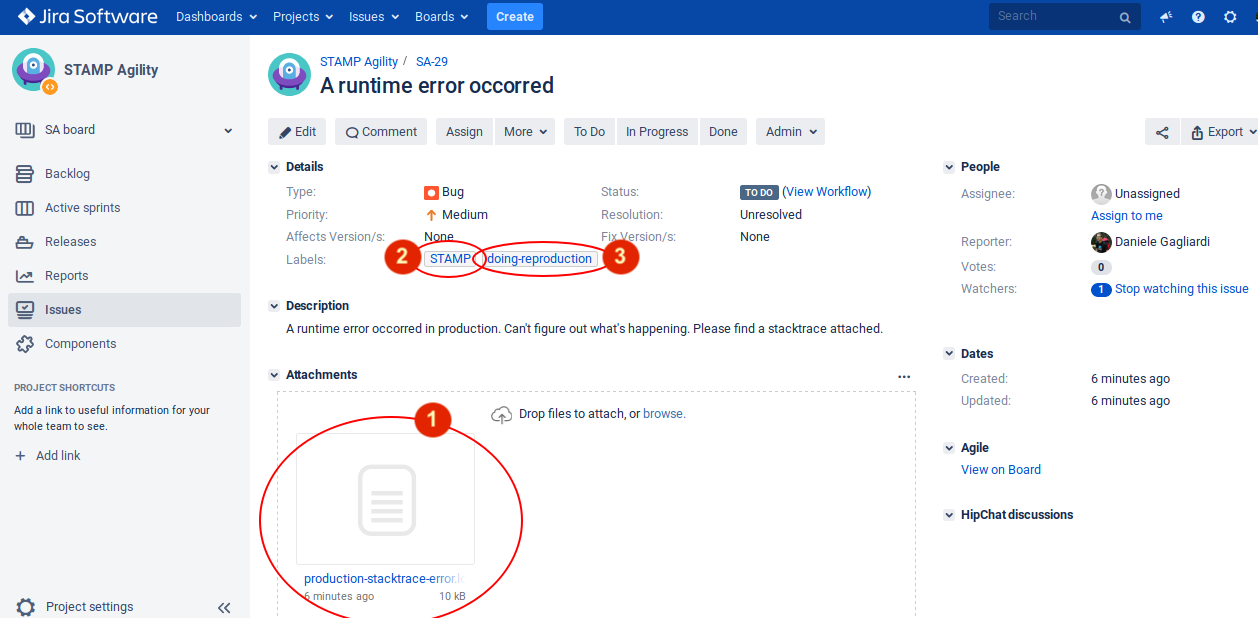
\includegraphics[width=0.8\textwidth]{conclusion/figures/deliverables_wp4_d44_images_jira-doing-reproduction.png}
    \caption{Triggering automatic crash reproduction with \botsing Jira plugin.}
    \label{fig:conclusion:botsingJira1}
\end{figure}

\begin{figure}
    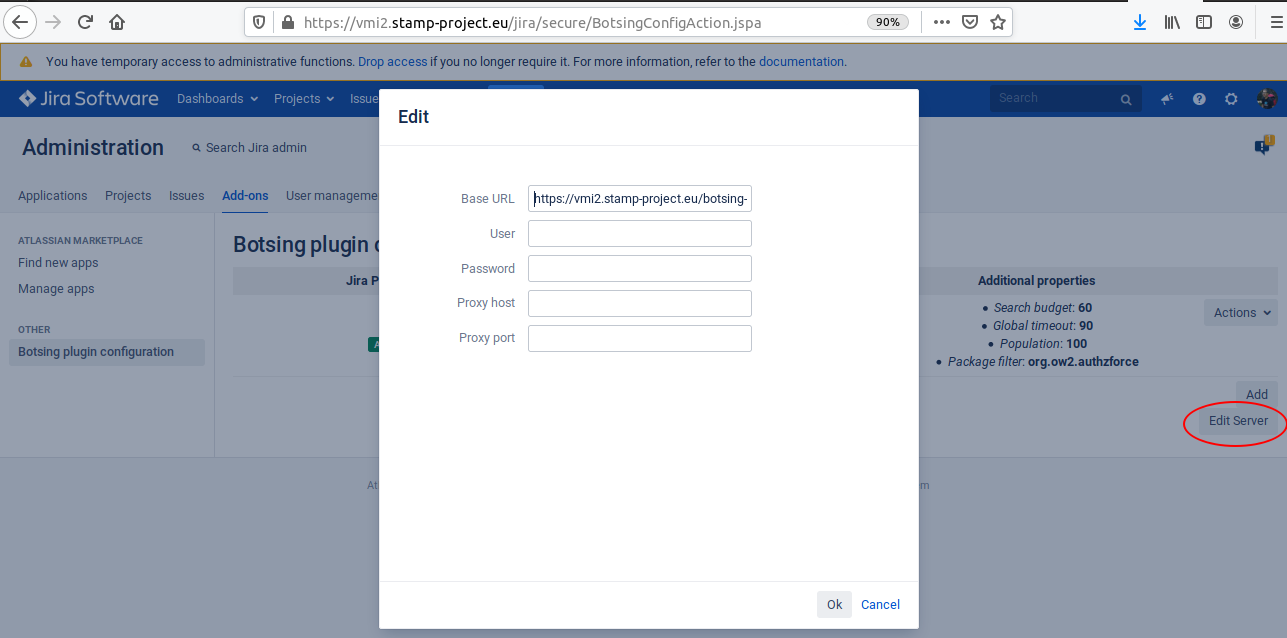
\includegraphics[width=0.8\textwidth]{conclusion/figures/deliverables_wp4_d44_images_jira-botsing-server-configuration.png}
    \caption{\botsing remote server configuration in Jira}
    \label{fig:conclusion:botsingJira2}
\end{figure}


\begin{figure}
    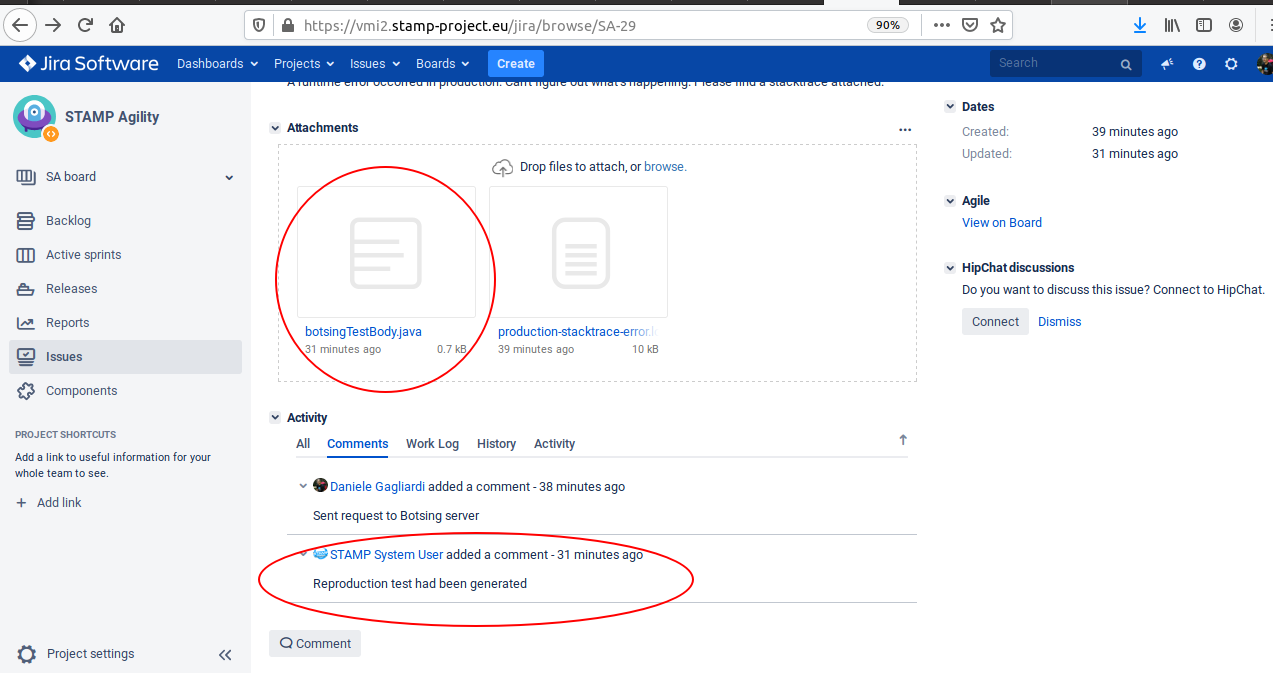
\includegraphics[width=0.8\textwidth]{conclusion/figures/deliverables_wp4_d44_images_jira-reproduction-done.png}
    \caption{crash reproducing test attached to the issue.}
    \label{fig:conclusion:botsingJira3}
\end{figure}


\begin{figure}
    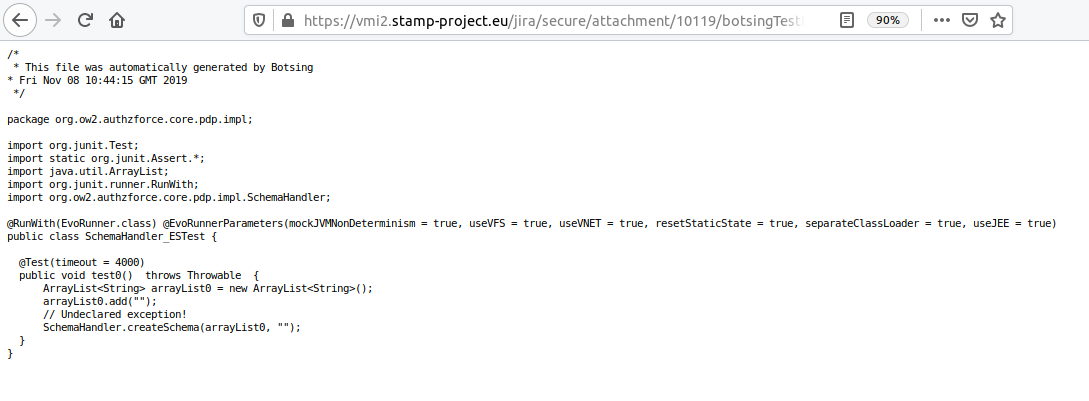
\includegraphics[width=0.8\textwidth]{conclusion/figures/deliverables_wp4_d44_images_jira-generated-test-case.png}
    \caption{A crash reproducing test case bu \botsing Jira plugin.}
    \label{fig:conclusion:botsingJira4}
\end{figure}

\textbf{\botsing Jira Plugin\footnote{This section uses the figures from STAMP's final deliverable: \url{https://github.com/STAMP-project/docs-forum/blob/master/docs/d44_final_api_public_version_services_courseware.pdf}}:}
In STAMP, our industrial partner implemented the \botsing Jira plugin \footnote{\url{https://github.com/STAMP-project/botsing-jira-plugin}}.
With this plugin, any software project using the Jira issue tracking system can automatically generate crash reproducing test cases for their reported crashes. The plugin automatically detects any issue with an attached stack trace (1 in Figure \ref{fig:conclusion:botsingJira1}), \texttt{doing reproduction} label and \texttt{STAMP} label (2 and 3 in Figure \ref{fig:conclusion:botsingJira1}) and initiates a \botsing instance in a remote server, linked in the configirations (look at Figure \ref{fig:conclusion:botsingJira2}), for reproducing the attached crash. 


The remote server attaches the crash reproducing test case to the issue after finishing the \botsing execution (Figure \ref{fig:conclusion:botsingJira3}). By clicking on the attachment, developers can see the crash reproducing test case (Figure \ref{fig:conclusion:botsingJira4}).



\subsubsection{\cling}

\cling is an open-source class-integration test generation tool for Java. It gets two classes, which are calling each other, and tries to generate tests covering different interactions between these two given classes. Section \ref{sec:cling:results} of this thesis has shown that this approach actually managed to detect the integration-level faults. 

In the same way as \evosuite, which has been used widely on industry \cite{almasi2017industrial} for generating unit-level tests, \cling has the potential to be used by software projects for generating integration-level tests complementing the tests generated by \evosuite. For this reason, we intend to implement different plugins for Maven, IntelliJ, and Jenkins to ease the application of \cling on different projects.

\subsubsection{Commonality Score For Unit Test Generation}
As mentioned in Section \ref{sec:cub:discussion}, we still need to perform a more in-depth investigation about the usefulness of commonality score in finding faults. However, since the introduced secondary objectives based on this metric aim to change how the statements are covered, we believe they can impact the test cases' understandability generated by the search process


\subsubsection{All tools unitedly}
The growths of the techniques introduced in this thesis will lead to a set of tools, alleviating developers from doing much groundwork in software testing. A developer can use each of these tools to generate a set of test cases/suites as a starting point for testing unit classes, class integrations, or debugging reported crashes. Since these approaches are automated, they take machine time, and that developer time can be spent on other tasks.  
Moreover, by new implementations and executions of the system under test, these approaches will have more data to improve their test generation and search guidance, and thereby, the benefits stemming from these approaches will increase as the software grows.

\section{Recommendations For Future Work}
This thesis shows that there are still many ways to improve the search-based test generation techniques for various criteria. Hence, this section gives some recommendations for future work.
\subsection{Search-based Crash Reproduction}

\subsubsection{R1: \CrashFunction improvements}
As described by section \ref{sec:background:evocrash:guidedalg}, the \CrashFunction fitness function is used in search-based crash reproduction to measure the distance of each generated test from throwing the same crash as the given one. The three elements in this fitness function may lead to flat landscapes in the search space. For instance, \textbf{the exception coverage} heuristic is a binary value, which indicates whether the same type of exception (as the given one) is thrown or not. Using only 0 and 1 for this heuristic can lead to a flat landscape in the search space.


\subsubsection{R2: Other secondary and helper objectives}
 Chapters \ref{sec:moho:introduction} and \ref{section:bbc:introduction} show how adding secondary objectives and helper-objectives help the existing \CrashFunction fitness function in reproducing more crashes. However, there are still many possibilities to improce the search objectives. First of all, the \CrashFunction fitness function itself can be modified to make sure that we have less flat landescapes in the search space. Also, more helper objectives can be combined with this fitness function to improve the exploration of the search process.



\subsection{Search-based Integration Testing}
\subsubsection{R3: Multiple classes integration}
In Chapter \ref{sec:cling:introduction}, we introduced a new search-based technique for testing interactions between two coupled classes. In the next step, this approach can be extended to handle more classes. It is even possible to design an approach to test the integration of two modules that contain multiple classes.

\subsection{Carving Knowledge For Search-based Test Generation}
This thesis showed the benefits of using the knowledge, collected from different sources, in search-based test generation. Hence, this section describes how the novel techniques, introduced in this thesis, can be extended.

\subsubsection{R4: Using more resources}
This thesis introduced various strategies to utilize the carved information from source code (\eg Chapter \ref{sec:cling:introduction}), existing test cases (\eg Chapter \ref{sec:model_seeding}), and execution logs (Chapter~\ref{sec:cub:intro}) in search-based test generation. However, other resources such as commits addressing previously detected faults can be used to generate more realistic test cases during the search process. Moreover, other useful information can be carved from the application's documentation.

\subsubsection{R5: Carving more information}
This thesis has used carved information from the method call sequences (\eg Chapters \ref{sec:model_seeding} and \ref{sec:moho:introduction}), call-site information (Chapter \ref{sec:cling:introduction}) and test execution patterns (Chapter \ref{sec:cub:intro}). Other data such as information regarding the input parameters can be carved for white-box search-based test generation to continue this research path. For example, some applications need strings, following a specific grammar and pattern (\eg XML, JSON), to be used in their testing. These kind of information can be carved from source code and documentation.